%%%%%%%%%%%%%%%%%%%%%%%%%%%%%%
% Section 3: Research Plan   %
%%%%%%%%%%%%%%%%%%%%%%%%%%%%%%
\section{Research Methodology}


\subsection{Theory Notes}

\mab{this is still just for private consumption. I'm writing down notes for the issues and I'm also going to be writing some research problems.
My next step is to define a research problem macro and write down some specific research problems.}

We begin with the stretch goal, which is coming up with an algorithmic model of the GPU.

\begin{rproblem}[\bf asymptotic GPU models]
We envision a single performance model for GPU computation.  With today's GPUs, however, a more realistic goal is a small set of algorithmic models to capture the different bottlenecks that GPUs face.
\end{rproblem}

Although there has been excitement about striving for a single algorithmic GPU model among parallel computing researchers~\cite{cite-stuff}, it is unlikely that there is a single performance model that works for all computations.

GPUs seem to defy efforts to model them elegantly. 
That said, often there are particular bottlenecks for a given problem, and for a single bottleneck one can model reasonably. 
Thus, part of our task, for each problem that we develop, is to determined what is the central computational bottleneck, and use and algorithmic model that captures that bottleneck.  Below we describe some of the models in which we will prove theorems


Surprisingly, a model as old as PRAM~\cite{cite-PRAM} is often predictive, despite being far from the GPU architecture. Syncs and global memory are the bottlenecks, but if the PRAM somehow behaves locally it can often work well enough.

Parallel external memory model (PEMM)~\cite{cite-PEMM}, or some variant, is elegant, and the idea of having increasing number of processors sharing increasing caches which have increasing cache lines is undoubtedly the right big picture.  But the model is still new and hasn't yet seen significant use, and it is unlikely that there is a direct transformation from a good PEMM model to a good

But not much has been done, and I feel these won't give you immediately super-good GPU algorithms

But one needs to worry about the other issues:

-Bank conflicts. There are some papers on these. These are sort of an anti-locality and seem orthogonal to how we normally make algorithms

-Memory vs parallelism. Each SM has a fairly small amount of shared memory. Normally GPUs are very good at, when a memory access need some cycles to return, brining in another warp of threads. Then one often has a bunch of warps running round-robin waiting in turn for their memory accesses to return. But, the more warps you assign to a thread, the less memory each gets. Finding the sweet spot here is very important in practice.

-Communication between threads in a warp. The 32 threads in a warp can communicate directly, and quickly, without going through shared memory. This leads to interesting algorithmic problems. For example, imagine an operation where thread $i$ gives row $i$ of a 32x32 matrix and receives column $i$ (one bit from each thread), what are the upper and lower bounds to sort? These questions are algorithmically beautiful but will likely lead to AKS-type results which will have no impact on practice. But, ignoring these operations ignores possible speedups.

-Synchronization. When we learn PRAM, there is a global sync after each step. If you code like this in a GPU you are in for a disaster. Global syncs are very expensive. Is there some elegant way to model this other than the obvious 1 sync = 1000 operations or something similar?



\begin{rproblem}[\bf peppermint flavored GPUs]
Make flavored GPUs that can be eaten. The challenge is that they are made of silicon, but that's better than a big mac.  
\label{rprob:peppermint}
\end{rproblem}

\begin{rproblem}[\bf General-purpose maplets and filters on GPUs]
Build compact, fast, distributed resizable, and general-purpose maplets (a filter where we can associate small values with keys) that scale to large datasets and exploit massive GPU parallelism. 
[Summary sentence talking a little bit about the state of the art and one about the challenges.]
\label{rprob:peppermint}
\end{rproblem}

Afterwards  we put in a couple of paragraphs talking about where we've used maplets effectively, where they still need to be used, etc.

\begin{rproblem}[\bf General-purpose hash table on GPUs]
Build compact, fast, distributed, resizable, and general-purpose hash table that scale to large datasets and exploit massive GPU parallelism. 
[Summary sentence talking a little bit about the state of the art and one about the challenges.]
\label{rprob:peppermint}
\end{rproblem}

\begin{itemize}
    \item It is hard to build resizesable filters and hash tables GPUs.
    \item Resizing is manual. You need an explicit call.  You need to do that from the host. 
    \item You need a runtime in GPU that can detect the space issue and reallocate dynamially.
    \item Theoretically, we can resize in more of an incremental way.
    \item We want the resizing to be automatically managed from the application's perspective. 
\end{itemize}


\begin{rproblem}[\bf Dynamic succinct data structures on GPUs]
Build dynamically updatable succinct data structures on GPUs.
[Summary sentence talking a little bit about the state of the art and one about the challenges.]
\label{rprob:peppermint}
\end{rproblem}

\begin{rproblem}[\bf Distributed data structures on multi-node GPUs]
Build distributed data structure that can achieve low variance across for load balancing, low communication volume and high communication bandwidth. 
[Summary sentence talking a little bit about the state of the art and one about the challenges.]
\label{rprob:peppermint}
\end{rproblem}

\prashant{Performance issues with distributed data sturctures}

\prashant{Load balancing, communication bandwidth, communication latency}


\subsection{Filters}
Applications require this:
\begin{itemize}
    \item Filters needs to associate small values with each item
    \item filter need to scale to large datasize and being able to saturate the GPU parallelism
    \item Support deletion of items to save space
    \item Being able to dynamically resize the filter
\end{itemize}

\subsection{Hash tables}
\begin{itemize}
    \item More locality and in turn performance
    \item variable-length keys and values support
    \item Being able to dynamically resize the filter
\end{itemize}

\subsection{Succinct/string string data structures}
SDSL library is heavily used across comp biology.

\begin{itemize}
    \item We need to build succinct data structures that are GPU-architecture aware.
    \item Making succinct data structures dynamic is hard. There is a trade off between space-efficiency and dynamism.
    \item We need to prove some lower-bounds to support dynamic operations while being succinct.
    \item We need to understand the empirical overheads to achieve dynamic operations.
\end{itemize}

\subsection{Trees}
\begin{itemize}
    \item Tree are relatively easier to distribute
    \item Tree have a fair amount of locality
    \item
\end{itemize}

\subsection{Distributed data structures}

\begin{itemize}
    \item more locality
    \item communication efficiency --- trade off between latency and bandwidth
    \item communication pattern -- all-to-all
    \item global coherence
\end{itemize}

\subsection{Spanning the entire hardware/software/network stack.}

\john{I don't think we want to say ``hardware'' here anywhere because we don't address it anywhere. ``Software stack'' makes more sense to me.}

\paragraph{Coverage areas.} Data structures are ubiquitous throughout the
hardware/software stack, as a way to connect heterogeneous components within a
system and to scale-out in data-center-scale applications.  AT has become a
bottleneck, but redesigning AT is tantamount to renegotiating the division of
labor among system components---requiring a closely knit team and an approach
that weighs the costs and benefits holistically.
Our team has the needed expertise:

% \begin{itemize}[noitemsep,nolistsep]
\begin{description}
  \item[Theory and Algorithms (PIs Bender and Farach-Colton)]
    Bender and Farach-Colton have written numerous
    top-tier theory
    publications~\cite{DBLP:conf/stoc/BenderFK19,DBLP:conf/focs/BenderFGJM018,DBLP:conf/soda/BenderCCFJT19,DBLP:conf/soda/AfshaniBFFGT17,DBLP:conf/pods/BenderFJMMPX17,DBLP:conf/stoc/BenderKPY16,DBLP:conf/soda/BenderFGKM17,DBLP:conf/pods/BenderBJKMPSSZ16}
    and have, along with collaborator Conway, made significant contributions in
    the theory of hashing and its
    applications~\cite{BenderFaGo18,BenderFaJo12,BenderFaJo11,PandeyBeJo17,PandeyAlBe18,PandeyBeJo18,PandeyBeJo17c,DBLP:conf/icalp/ConwayFS18}.


    \item[GPU Systems (PIs Owens and Pandey)] Owens's research program in GPU computing~\cite{Owens:2007:ASO,Owens:2008:GC} spans nearly 20 years and includes representative research advances in fundamental algorithms~\cite{Sengupta:2007:SPF}, data structures~\cite{Lefohn:2006:GGE,Alcantara:2009:RPH}, performance engineering~\cite{Zhang:2011:AQP}, programming models~\cite{Gupta:2012:ASO, Tzeng:2010:TMF}, and applications~\cite{Wang:2017:GGG}.

    \item[High-Performance Computing (PIs Bender, Farach-Colton, Owens, and
        Pandey)] Bender, Farach-Colton, Owens, and Pandey have
      written a number of top-tier papers in HPC~\cite{pandey2020timely,bender2017two,eckstein2015pebbl,agrawal1989four,bender2008communication,greenberg1999enabling},
      and had considerable impact on HPC practice.  PI Bender's and Phillips
      work in HPC has focused on scheduling and  won a joint R\&D 100 Award for
      processor scheduling and allocation algorithms, which were licensed by
      Cray and incorporated into SLURM.  PIs Bender and Farach-Colton's company
      Tokutek deployed software to manage metadata in a large cloud storage
      service. Owens led the first implementation of MPI on GPUs~\cite{Stuart:2009:MPO:withouturl,Stuart:2011:EMT}, the first multi-GPU MapReduce~\cite{Stuart:2011:MMO}, and more recent work on scalable graph analytics on HPC machines~\cite{Pan:2018:SBS,Pan:2017:MGA,Chen:2022:SIP}.

    \item[Large-scale genomics (PIs Bender, Farach-Colton, and Pandey)]

\end{description}


\paragraph{Target distributed applications and systems, and the heterogeneous platforms on which they run.}

Accelerating data analyses will benefit all big-data application domains.  In
this proposal, we will primarily focus on \textbf{genomics} applications. We will
start with scalable graph processing applications (e.g.,
Graph500~\cite{graph500}), and will then explore data-serving applications
(e.g., key-value stores~\cite{lakshman2010cassandra, papyruskv-kim-sc17} and
databases~\cite{MySQL}), followed by data-analytics frameworks (e.g., Apache
Spark~\cite{Zaharia:Spark:HotCloud10}). To understand the benefits and the
implications on massively parallel scale-out systems, we will study traditional
scientific simulations, such as molecular simulations (e.g., GTC~\cite{GTC}) and
biomolecular workflows (e.g., Gromacs~\cite{GROMACS}), followed by modern HPC ML
suites (e.g., MLPerf~\cite{MLPerf}).

\paragraph{Notions of Scale.}  Our proposed work address several notions of
scale.  First, virtual memory is a major bottleneck for scaling individual
machines to larger memories and CPU counts.  Without a principled redesign of
VM, additional RAM and cores will be of diminishing value.  Second, our work
supports \emph{scale-out} cloud applications, which rely on naming, placing, and
translating accesses to resources that are distributed across multiple machines.
%Currently, if one needs to do complex operations on sensitive data in the
%cloud, there is no secure and sensible option other than scaling out across
%multiple SGX enclaves.
If successful, our work will improve the performance of each node, as well as
the working-set size each node can handle, potentially improving both by orders
of magnitude.  Third, this includes scaling from only CPUs, to {\em
heterogeneous} computing accelerators, such as GPUs and FPGAs, at rack-scale or
greater.  Prior work has demonstrated that data movement and address translation
in GPUs is a first-order performance issue~\cite{pichai:gpu,
power:gpummu,rossbach:ptask}. Further, cloud computing infrastructure, such as
Microsoft's Catapult, aggregate these accelerators and move data  at the
granularity of racks, not single nodes~\cite{putnam:catapult}.  These
accelerators are evolving rapidly and in ways that are hard to anticipate; thus,
a principled design is necessary to efficiently scale to new classes of future,
unknown compute hardware.


\subsection{A component of your plan}

% 
\setlength\intextsep{0pt}
\begin{wrapfigure}[20]{R}{2.4in}
\vspace{-5pt}
\centering
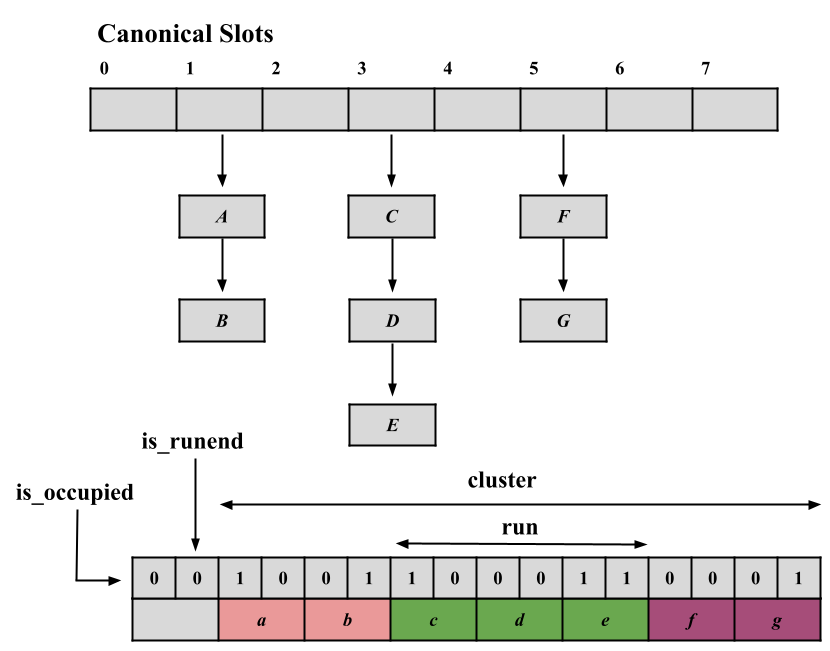
\includegraphics[width=2.4in]{images/canonical_slots}
\caption{Quotient filter block diagram.}
\label{fig1}
\end{wrapfigure}




\begin{wraptable}[15]{r}[0.01in]{4.5in}
\label{table1}
\caption{A sample table wrapped by text.}
\begin{center}
\vspace{-10pt}
\scriptsize
\begin{tabular}{  c  c  c  }
\hline
\hline
Stability & $M_u$ & $M_{\tau}$ \\
\hline\hline\\
Neutral & $\cfrac{z}{z_\Delta} - \cfrac{\ln(z/z_o)}{\ln(z_\Delta/z_o)}$ & $\cfrac{z}{z_\Delta} - \cfrac{1}{\ln(z_\Delta/z_o)}$\\\\
\hline \\
Stable & $\left(1 - \cfrac{\Psi}{2}\right)\cfrac{z}{z_\Delta} - \left(1 - \cfrac{\Psi_\Delta}{2}\right)
\left(\cfrac{\ln(z/z_o)-\Psi}{\ln(z_\Delta/z_o)- \Psi_\Delta}\right)$ & $\cfrac{z}{z_\Delta} - \cfrac{\left(1 - \cfrac{\Psi_\Delta}{2}\right)}{\ln(z_\Delta/z_o) - \Psi_\Delta}$\\\\
\hline \\
Unstable & $\cfrac{4}{3}\left[\left(\cfrac{1-x^3}{1-x_{\Delta}^{4}}\right) -  \left(\cfrac{1-x_{\Delta}^3}{1 - x_{\Delta}^{4}}\right)\left(\cfrac{\ln(z/z_o)-\Psi}{\ln(z_\Delta/z_o)- \Psi_\Delta}\right)\right]$ & $\cfrac{z}{z_\Delta} - \cfrac{\cfrac{4}{3}\left(\cfrac{1-x_{\Delta}^3}{1 - x_{\Delta}^{4}}\right)}{\ln(z_\Delta/z_o) - \Psi_\Delta}$\\\\
\hline
\hline
\end{tabular}
\end{center}
\end{wraptable}



% I found it useful to include a summary of the proposed work
% given in each subsection to help out reviewers.
\subsubsection{Specific tasks for this research component}
\begin{itemize}
\setlength\itemsep{0em}
\item Do a thing and blow your mind
\item Question your life choices
\item Drink coffee
\end{itemize}

\begin{center}
\begin{minipage}{.3\textwidth}
\begin{equation}
 \bar u = \bar u_{ll} + u_* \beta M_{u} \label{new_u}
\end{equation}
\end{minipage}
\begin{minipage}{.36\linewidth}
\begin{equation}
  \tau_{xz} = u_* u_{*ll} + \kappa u_*^2 \beta M_{\tau} \label{new_tau} \mbox{ ,}
\end{equation}
\end{minipage}
~\\Sample equations that consume minimal space.
\end{center}


